% !TeX spellcheck = ru_RU
% !TEX root = main.tex

%\begin{figure}[t]
%\centering
%\includegraphics{graph2.pdf}
%\caption{The Second Set of Benchmarks}
%\label{eval:second}
%\end{figure}

\section{Оценка производительности}
\label{sec:evaluation}

Изначально, с помощью тестирования производительности мы хотели оценить, какое влияние оказывает выбор языка OCaml для реляционного программирования.
В дополнении к этому, реляционное программирование было реализовано эффективно с помощью отказа от тегирования, и влияние этого решения тоже должно быть оценено.
Для сравнения был выбрана реализация faster-miniKanren\footnote{\url{https://github.com/michaelballantyne/faster-minikanren}} для Scheme/Racket.
В OCanren были реализованы
оптимизации~\cite{WillThesis},% Выпилен Personal Communications по причине шаблона ИСП РАН
%оптимизации~\cite{WillThesis, Optimizations},
которые применяются в faster-miniKanren.
Также была проведена работа по обеспечению обхода дерева поиска одинаковым образом.
%
%One of our initial goals was to evaluate what performance impact would choosing OCaml as a host language makes.
%In addition we spent some effort in order to implement \miniKanren in an efficient, tagless manner, and, of course, the outcome of this decision also has to be
%measured. For comparison we took faster-miniKanren\footnote{\url{https://github.com/michaelballantyne/faster-minikanren}}~--- a full-fledged \miniKanren{} implementation for Scheme/Racket.
%It turned out that faster-miniKanren implements a number of optimizations~\cite{WillThesis, Optimizations} to speed up the search; moreover, the search order in our implementation initially was a little bit different.
%In order to make the comparison fair, we additionally implemented all these optimizations and adjusted the search order to exactly coincide with
%what faster-miniKanren does.

\begin{figure}[t]
\centering
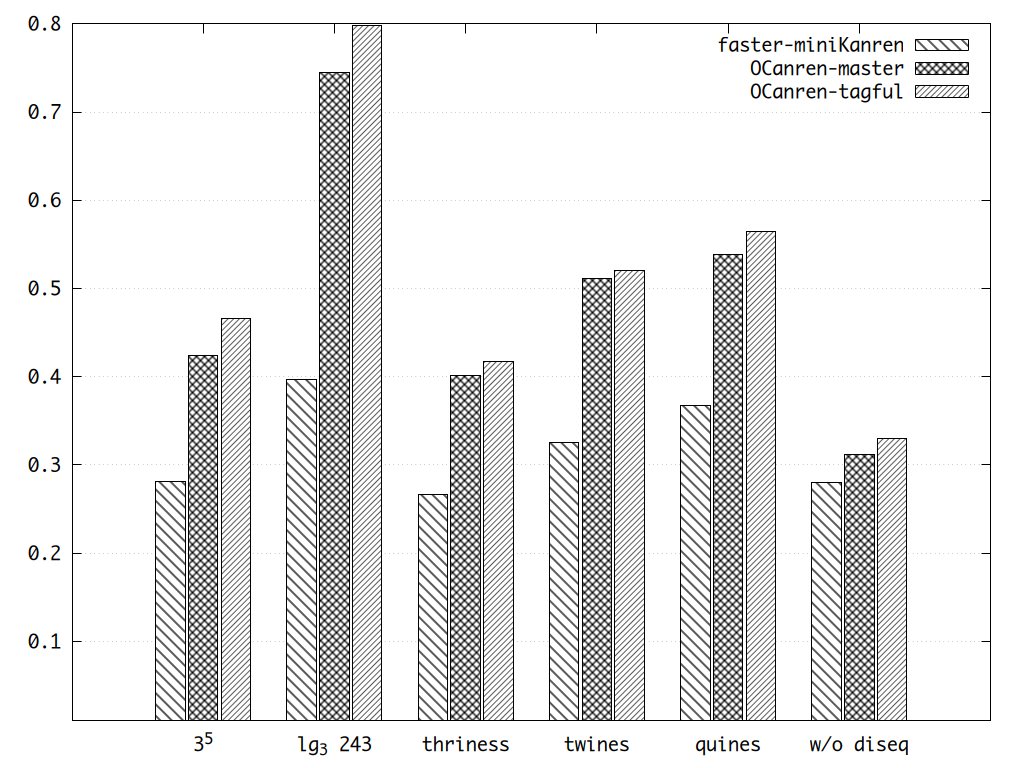
\includegraphics[scale=0.8]{graph.png}
\caption{Результаты оценки производительности}
\label{eval}
\end{figure}

\FloatBarrier

Для набора тестов были выбраны следующие задачи:
%For the set of benchmarks we took the following problems:

\begin{itemize}
\item \textbf{pow, logo}~--- реляционное возведение в степень и логарифмирование~\cite{KiselyovArithm} чисел в двоичном представлении.
Конкретно выбраны $3^5=243$ и $log_3 243=5$.
%and logarithm for integers in binary form. The concrete tests relationally computed
%$3^5$ (which is 243) and $log_3 243$ (which is, conversely, 5). The implementaion was adopted from~\cite{KiselyovArithm}.
\item \textbf{quines, twines, trines}~--- программы, вычисляющиеся в себя, использованные для тестирования реляционных интерпретаторов~\cite{Untagged}.
Конкретно тесты вычисляю первые 100, 15 и 2 ответа(ов) для соответствующих задач.
%\item \textbf{quines, twines, trines}~--- self/co-evaluating program synthesis problems from~\cite{Untagged}. The
%concrete tests took the first 100, 15 and 2 answers for these problems respectively.
\end{itemize}

%Since the last bundle of benchmarks uses disequality constraints (and, hence, $\mu$Kanren is ruled out) we
%split all benchmarks into two sets.

Вычисления производились на компьютере с процессором Intel Core i7-4790K CPU @ 4.00GHz и 16GB памяти.
Для OCanren использовался компилятор \texttt{OCaml-4.14.2+flambda}, для faster-miniKanren~--- Chez~Scheme~9.5.8.
Все бенчмарки компилировались в нативный код и вычислялось среднее время за 40 испытаний.
Результаты представлены на рисунке~\ref{eval}.
Репозиторий с кодом и инструкции по воспроизведению эксперимента доступны на GitHub\footnote{\url{https://github.com/Kakadu/ocanren-perf/tree/ispras-paper2025}}.
%All benchmarks were executed in the natively compiled mode ten times, then average user time was taken. The results of the evaluation
%are shown on Figure~\ref{eval}. The whole evaluation repository with all scripts and detailed description is accessible
%from \lstinline|GitHub|\footnote{\url{https://github.com/Kakadu/ocanren-perf/tree/ispras-paper2025}}.

Наблюдения показывают, что важность нетегированного представления варьируется от задачи.
В зависимости от видов термов, участвующих в унификации, прирост производительности будет разниться.
Действительно, если термы являются копиями друг друга, то унификации нужно совершить полный обход термов. Если же термы не равны, то унификация может завершиться раньше, без полного обхода термов.
%The first conclusion, which is rather easy to derive from the results, is that the tagless approach indeed matters. Our initial
%implementation did not show essential speedup in comparison even with $\mu$Kanren (and was even \emph{slower} on the logarithm
%and permutations benchmarks). The situation was improved drastically, however, when we switched to the tagless version.

Также стоит отметить, что реализация на OCaml отстаёт по сравнению с реализацией для Chez Scheme. Вероятно, это связано с особенностями хранения данных~\cite{BIBOP94} в реализации компилятора. Детальное исследование различий сред исполнения OCaml и Scheme оставлено на будущее.
%Yet, in comparison with faster-miniKanren, our implementation is still lagging behind. We can conclude that the optimizNfr;tations
%used in the Scheme/Racket version, have a different impact in the OCaml case; we save this problem for future research.

